
\documentclass[french,twoside]{book}
\usepackage[utf8]{inputenc}
\usepackage[T1]{fontenc}
\usepackage[french]{babel}
\usepackage{lmodern}
%-------------------------------------------------------------------------- 
% frenchb de babel change les points en tirets, retour à l'original :
\frenchbsetup{ItemLabeli=$\bullet$}
%--------------------------------------------------------------------------
% Utilitaires
%--------------------------------------------------------------------------
% Packages mathématiques
\usepackage{amsmath}
\usepackage{amsfonts}
\usepackage{amssymb}
\usepackage{amsthm}
\usepackage{bold-extra}
%--------------------------------------------------------------------------
%Graphismes
\usepackage{graphicx}%Pour l'inclusion d'images
\usepackage{tikz}%Pour les dessins divers (arbres, graphes...)
\usetikzlibrary{calc}
\usepackage{multicol}%pour du texte sur plusieurs colonnes
%--------------------------------------------------------------------------
%Pour mettre en page des exercices facilement 
\usepackage[lastexercise]{exercise}
\renewcommand{\ExerciseName}{Question}
\renewcommand{\ExerciseHeaderTitle}{\ ---\quad\textbf{\textsc{\ExerciseTitle}}}
\renewcommand{\ExerciseHeader}{\vspace{0cm}\noindent\textbf{\ExerciseName\ \ExerciseHeaderNB}\ \ExerciseHeaderDifficulty\ExerciseHeaderTitle\par}

\renewcommand{\AnswerHeader}{\noindent\textbf{Solution de la question \ExerciseHeaderNB{} - }} 
\newcounter{exo}
\setcounter{exo}{0}
%--------------------------------------------------------------------------
\newif\ifcaml \camlfalse
\usepackage{listings}
% Configuration des listings
\lstset{escapechar = §,%
        frameround=tttt, frame = lines, linewidth=0.95\textwidth,%
        xleftmargin=0.025\textwidth,%
        breaklines=true,% 
        showstringspaces=false,%
       }
\lstset{
literate = {à}{{\`a}}1
           {À}{{\`A}}1
           {â}{{\^a}}1
           {ç}{{\c c}}1
           {Ç}{{\c C}}1
           {é}{{\'e}}1
           {É}{{\'E}}1
           {è}{{\`e}}1
           {È}{{\`E}}1
           {ê}{{\^e}}1
           {Ê}{{\^E}}1
           {ï}{{\"i}}1
           {î}{{\^i}}1
           {ô}{{\^o}}1
           {œ}{{\oe}}1
           {ù}{{\`u}}1 
           {ÿ}{{\"y}}1
       }
\renewcommand{\lstlistingname}{Programme}
\lstset{keywordstyle=\bfseries,%
       commentstyle=\itshape,% 
       stringstyle=,% 
       basicstyle=\ttfamily
      }
\ifcaml
  \lstset{tabsize = 2,%
          language=caml,%
         }
\else
  \lstset{tabsize = 4,%
          language=python,%
          morekeywords={as, assert, False, None, nonlocal, True, with, 
                        yield,float, int, abs, type}
          }
\fi
%--------------------------------------------------------------------------
\newtheoremstyle{definition}%
{}{}%
{\itshape}{}%
{\bfseries}{}%
{\newline}%
{\thmname{#1 : }\thmnumber{}\thmnote{#3}}
\theoremstyle{definition}
\newtheorem*{defin}{Définition}
\newtheorem*{thm}{Théorème}
%--------------------------------------------------------------------------
% Diverses fonctions
%--------------------------------------------------------------------------
\def\Vec#1{\overrightarrow{#1}}
\def\norme#1{\left\| #1 \right\|}
\def\C{{\mathbb C}}
\def\K{{\mathbb K}}
\def\M{{\cal M}}
\def\N{{\mathbb N}}
\def\Q{{\mathbb Q}}
\def\R{{\mathbb R}}
\def\Z{{\mathbb Z}}
\def\tr{{\rm tr}}
\def\trans#1{\,{\vphantom{#1}}^t\!#1\/}
\def\type#1{\text{\normalfont\ttfamily #1}}
\def\Type#1{{\normalfont\bfseries\ttfamily #1}}
\let\le=\leqslant 
% remplace le inférieur ou égal avec barre horizontale par une barre oblique
\let\ge=\geqslant 
% remplace le supérieur ou égal avec barre horizontale par une barre oblique
%--------------------------------------------------------------------------
% Présentation
%--------------------------------------------------------------------------
% Je n'aime pas les indentations de paragraphe :
\parindent=0pt
%--------------------------------------------------------------------------
%--------------------------------------------------------------------------
% Configuration de la page
%--------------------------------------------------------------------------
%--------------------------------------------------------------------------
%Taille des marges
\usepackage[a4paper,left=3cm,right=3cm,top=3cm,bottom=3cm]{geometry}
%--------------------------------------------------------------------------
% En-tête de chapitre (les différents poly)
\usepackage[explicit]{titlesec}
\titleformat{\chapter}[display]{\Large\bfseries}
            {\filright {\scshape\huge  D.S. \numero}}{0pt}
            {\titlerule \vspace{2ex}
             \filleft\sffamily\bfseries
               {\fontsize{50}{55}\usefont{T1}{qcs}{m}{sc}\selectfont #1}
            }
            [\vspace{2ex}\titlerule]

\titlespacing*{\chapter}{0pt}{0pt}{3cm}
%--------------------------------------------------------------------------
% Choix de la numérotation
\renewcommand{\thechapter}{\Roman{chapter}}
\renewcommand{\thesection}{\arabic{section}}
%--------------------------------------------------------------------------
%Configuration des en-têtes et bas-de-pages
\usepackage{fancyhdr}
% Le style pour les polys info sup
\pagestyle{fancy}
% Voici les commandes pour les intitulés leftmark, rightmark)
\renewcommand{\chaptermark}[1]{\markboth{\thechapter. {\sc #1}}{} }
\renewcommand{\sectionmark}[1]{\markright{\thechapter.\thesection-#1}{} }
% Hauts de page, O/E pour impair/pair (odd/even)
%                L/R pour gauche droite
\fancyhead[RO, LE]{DS \numero}% Pages impaires haut gauche : section
\fancyhead[LO,RE]{\classe}
% bas de page, mêmes positions
\fancyfoot[LO,RE]{}
\fancyfoot[LE,RO]{}
\fancyfoot[C]{\thepage}
\renewcommand{\headrulewidth}{0.2pt}% Ligne en haut
\renewcommand{\footrulewidth}{0pt}% pas en bas
%-------------------------------------------------------------------------- 
\renewcommand{\thefigure}{\arabic{figure}}
%-------------------------------------------------------------------------- 
% Pour les premières pages, on peut imposer un style vide
% en écrivant *\thispagestyle{empty}* après le chapitre
%--------------------------------------------------------------------------
\newenvironment{abstract}{\begin{minipage}{0.2\linewidth} {\Large \bf Objectifs} \end{minipage}
\begin{minipage}{0.75\linewidth}\itshape} {\end{minipage}}
%--------------------------------------------------------------------------
% Personnalisations générales
\title{D.S. d'informatique}
\date{2018-2019}

\usetikzlibrary[automata]\def\numero{1+}
\def\classe{Option info MP1}

\camltrue
%-------------------------------------------------------------------------------
%-------------------------------------------------------------------------------
%-------------------------------------------------------------------------------
\begin{document}
%-------------------------------------------------------------------------------
%-------------------------------------------------------------------------------
%-------------------------------------------------------------------------------
\chapter{Arborescences}
%-------------------------------------------------------------------------------
%-------------------------------------------------------------------------------
%-------------------------------------------------------------------------------
\section{Première partie}
%-------------------------------------------------------------------------------
%-------------------------------------------------------------------------------
%-------------------------------------------------------------------------------
\begin{Exercise}
On compte $N_t(1,1) =3$, $N_t(1,2) =4$, $N_t(1,3) =0$, $N_t(2,2) =1$, $N_t(2,3) =1$, $N_t(1) =10$, $N_t(2) =7$ et $N_t(3) =2$. La matrice de ramification est donc $\begin{pmatrix}
  1    &   0 &  0  \\  \frac 47   &  \frac 37  & 0   \\  0  & \frac 12   &  \frac 12\end{pmatrix}$.
\end{Exercise}
%--------------------------------------------------------------------------
%-------------------------------------------------------------------------------
\begin{Exercise}
Les arêtes d'épaisseur $k$ parviennent à un nœud qui peut être de bi-épaisseur $(k-1, k-1)$ ou $(i, k)$ avec $i < k$ pour $k\ge 1$. On a donc $\displaystyle N_t(k) = \sum_{i=1}^{k-1} N_t(i,k)+ N_t(k,k)$ ce qui implique que $\displaystyle \sum_{i=0}^{ep(t)} R_{k,i} = 1$ pour $k> 1$ ; l'égalité pour $k=1$ est évidente. 
\end{Exercise}
%--------------------------------------------------------------------------
%-------------------------------------------------------------------------------
\begin{Exercise}
La question est ambiguë : que signifie "remplis" ?

Si on interprète "le niveau de profondeur $h$ est rempli" par "tous les nœuds de niveau $h-1$ ont deux fils c'est-à-dire sont de degré 2 alors cela est équivalent au fait qu'il n'y a pas de feuille au niveau $h-1$ (car les nœuds ont 0 ou 2 pour degré) donc que toutes les feuilles sont au niveau maximal.

Dans ce cas on montre par récurrence que tous les nœuds de profondeur $k$ on une bi-épaisseur $(h-k, h-k)$ car alors les arêtes entre les nœuds de profondeur $k$ et ceux de profondeur $k-1$ ont pour épaisseur $h - k +1$. On a ainsi $N_t(i, j)= 0$ pour $i\ne j$.

On en déduit que $ep(t) = h+1$ car l'épaisseur de la racine est $(h,h)$ :

 la matrice de bifurcation est $I_{h+1}$.
\end{Exercise}
%--------------------------------------------------------------------------
%-------------------------------------------------------------------------------
\begin{Exercise} Un arbre-peigne de hauteur $h$ a $h$ nœuds internes, chacun ayant un fils feuille (2 pour le dernier). La bi-épaisseur du dernier nœud et $(1,1)$ tandis que les autres ont la bi-épaisseur $(2,1)$. On a donc $N_2 = h$, $N_{2,1}=h-1$ et $N_{1,1} = 1$ donc la matrice d'adjacence vaut $\begin{pmatrix} 1&0 \\ \frac{h-1}h&\frac 1h \end{pmatrix}$.
\end{Exercise}
%--------------------------------------------------------------------------
%-------------------------------------------------------------------------------
\begin{Exercise}
	On remarque d'abord que l'épaisseur d'un arbre semble mesurer la densité des n{\oe}uds de degré 2 : plus l'arbre est effilé moins l'épaisseur est importante On voit aussi que l'apparition d'arêtes d'épaisseur importante demande des n{\oe}uds d'épaisseur de la forme $(k, k)$ : la matrice aura des termes diagonaux dominants 
\end{Exercise}
%--------------------------------------------------------------------------
%-------------------------------------------------------------------------------
\begin{Exercise}
	Un arbre de taille $n\ge 1$ admet au moins un n{\oe}ud terminal qui aura donc une bi-épaisseur $(1,1)$  ainsi il existe toujours une arête d'épaisseur 2 On a vu que les arbres peignes avaient une épaisseur 2 ; ainsi $\lambda(n) = 2$.
	
	Pour obtenir une épaisseur 2 il faut que tous les n{\oe}uds aient $(1,1)$ ou $(1,2)$ comme bi-épaisseur. En particulier un arbre de hauteur $n$ admet au moins un fils d'épaisseur 1 donc une feuille, l'autre étant un arbre de hauteur $n-1$ et d'épaisseur 2 au plus. Si on note $\mu(n)$ le nombre d'arbres de hauteur $n$ et d'épaisseur 2 on a donc $\mu(1) = 1$ et $\mu(n) = 2\mu(n-1)$ car on choisit le fils de hauteur $n-1$. On aboutit à $\mu(n)=2^{n-1}$, c'est en fait le nombre d'arbres-peignes.
\end{Exercise}
%--------------------------------------------------------------------------
%-------------------------------------------------------------------------------
\begin{Exercise}
	Un arbre complet de hauteur $h-1$ admet $2^{h}-1$ n{\oe}uds  et son épaisseur est$ h$. De plus, une épaisseur $h$ n'est possible que s'il existe un n{\oe}ud de bi-épaisser $(h-1, h-1)$ donc deux  n{\oe}uds d'épaisseur $h-1$ d'où, par récurrence, $2^{h-1}$ n{\oe}uds terminaux de bi-épaisseur $(1,1)$. Ainsi un arbre d'épaisseur $h$ admet au moins $\displaystyle \sum_{k=0}^{h-1}2^k=2^h-1$ n{\oe}uds : on a $n(h) \ge 2^h-1$ avec la borne atteinte.

Si on considère un arbre-peigne de taille $p$ et que l'on remplace une feuille par un arbre complet de hauteur $h-1$ on obtient un arbre d'épaisseur $h$ et de taille $p+ 2^h -1$ donc il n'y a pas de majorant possible pour $n(h)$.

Les valeurs possibles pour $n(h)$ sont donc les entiers supérieurs ou égaux à $2^h - 1$.
\end{Exercise}
%--------------------------------------------------------------------------
%-------------------------------------------------------------------------------
\begin{Exercise}
Pour stocker une structure arborescente on doit stocker, pour chaque n{\oe}ud, les informations relatives au n{\oe}ud ainsi que qu'un moyen de déterminer ses fils. L'encombrement en mémoire est donc proportionnel au nombre de n{\oe}uds, indépendamment du langage.

En Caml, un typage minimal possible est
\begin{lstlisting}
type forme_a = Vide|Noeud of forme_a  * forme_a;;
\end{lstlisting}
\end{Exercise}
%--------------------------------------------------------------------------
%-------------------------------------------------------------------------------
\begin{Exercise}
\begin{lstlisting}
let rec epaisseur arbre = 
  match arbre with
  |Vide -> 1
  Noeud(g, d) -> let eg = epaisseur g in
                    let ed = epaisseur d in
                    if eg = ed then eg + 1 else max eg ed ;;
\end{lstlisting}
\end{Exercise}
%--------------------------------------------------------------------------
%-------------------------------------------------------------------------------
\begin{Exercise}
La fonction existe en OCaml : c'est \type{Random.random}.
On commence par une fonction de choix, une variable aléatoire suivant une loi de Bernoulli de paramètre $0,5$.
\begin{lstlisting}
let choix () = Random.random() < 0.5;;
\end{lstlisting}

On écrit la fonction d'ajout d'un n{\oe}ud : 
\begin{lstlisting}
let rec ajout arbre = 
  match arbre with
  |Vide -> Noeud(Vide, Vide)
  Noeud(g, d) -> if choix()
                 then Noeud(ajout g, d)
                 else Noeud(g, ajout d);;
\end{lstlisting}

\newpage

On peut enfin ajouter $n$ n{\oe}uds à un arbre vide :
\begin{lstlisting}
let creation n = 
  let arbre = ref Vide in
  for i = 1 to n do
    arbre := ajout !arbre done;
  !arbre;;
\end{lstlisting}
Au pire, lors de la création d'un arbre-peigne, la complexité, en nombre d'appels récursifs sera $\displaystyle \sum_{k=0}^{n-1} k$, c'est un ${\cal O}(n^2)$.
\end{Exercise}
%--------------------------------------------------------------------------
%-------------------------------------------------------------------------------
\begin{Exercise}La question est mal rédigée :
\begin{itemize}
    \item elle n'utilise pas la matrice
    \item elle ne précise rien sur $r2_k$, qui devrait s'appeler plutôt $r2(k)$.
\end{itemize}

Un algorithme possible serait alors
\begin{lstlisting}
entrée : une matrice M
s est le nombre de ligne de M
t est un arbre avec 1 nœud, d'épaisseur s
tant qu'il reste des feuille d'épaisseur différente de 1
    choisir une telle feuille f
    k est son épaisseur
    i = r2(k)
    si i = k
        alors a = k, b = k
        sinon si r1() < 0.5
            alors a = i, b =k
            sinon a = k, b = 1
    ajouter une feuille d'épaisseur a comme fils gauche de f        
    ajouter une feuille d'épaisseur b comme fils droit de f        
\end{lstlisting}
 On a tiré au sort les tailles des fils pour ne pas déséquilibre l'arbre.
 
Si la probabilité de $r2(k)=1$ n'est pas nulle l'algorithme pourrait ne pas terminer mais la probabilité que le nombre d'étape soit supérieur à $N$ tend vers 0 quand $N$ grandit sauf si $r2(k)=1$ est de probabilité 1.
\end{Exercise}
%--------------------------------------------------------------------------
%-------------------------------------------------------------------------------
\begin{Exercise}
L'hypothèse faite est que $r2$ dépende aussi de $M$ avec $P\bigr(r2(k, M) = i\bigl) = M_{k, i}$.

Dans ce cas on peut imaginer que l'arbre construit (si l'algorithme termine) aura une matrice de ramification proche de $M$.
\end{Exercise}
%-------------------------------------------------------------------------------
\newpage
%-------------------------------------------------------------------------------
%-------------------------------------------------------------------------------
\section{Deuxième partie}
%-------------------------------------------------------------------------------
%-------------------------------------------------------------------------------
%-------------------------------------------------------------------------------
\begin{Exercise} Évaluation de gauche à droite de $a+(b-c)*(d-e)$.
  \begin{center}
    \begin{tabular}{l|c|c|c|c}
       instruction&$R_0$&$R_1$&$R_2$&$R_3$ \\
       \hline
       $R_0 \leftarrow a$& $a$&&&\\
       $R_1 \leftarrow b$& $a$&$b$&&\\
       $R_2 \leftarrow c$& $a$&$b$&$c$&\\
       $R_1 \leftarrow R_1-R_2$& $a$&$b-c$&$c$&\\
       $R_2 \leftarrow d$& $a$&$b-c$&$d$&\\
       $R_3 \leftarrow e$& $a$&$b-c$&$d$&$e$\\
       $R_2 \leftarrow R_2-R_3$& $a$&$b-c$&$d-e$&$e$\\
       $R_1 \leftarrow R_1*R_2$& $a$&$(b-c)*(d-e)$&$d-e$&$e$\\
       $R_0 \leftarrow R_0+R_1$& $a+(b-c)*(d-e)$&$(b-c)*(d-e)$&$d-e$&$e$\\
    \end{tabular}
  \end{center}
On utilise 4 registres
\end{Exercise}
%--------------------------------------------------------------------------
%-------------------------------------------------------------------------------
\begin{Exercise}
 Évaluation de droite à gauche de $a+(b-c)*(d-e)$.
  \begin{center}
    \begin{tabular}{l|c|c|c|c}
       instruction&$R_0$&$R_1$&$R_2$&$R_3$ \\
       \hline
       $R_0 \leftarrow e$& $e$&&&\\
       $R_1 \leftarrow d$& $e$&$d$&&\\
       $R_0 \leftarrow R_1-R_0$& $d-e$&$d$&&\\
       $R_1 \leftarrow c$& $d-e$&$c$&&\\
       $R_2 \leftarrow b$& $d-e$&$c$&$b$&\\
       $R_1 \leftarrow R_2-R_1$& $d-e$&$b-c$&$b$&\\
       $R_0 \leftarrow R_1*R_0$& $(b-c)*(d-e)$&$b-c$&$b$&\\
       $R_1 \leftarrow a$& $(b-c)*(d-e)$&$a$&$b$&\\
       $R_0 \leftarrow R_0+R_1$& $a+(b-c)*(d-e)$&$a$&$b$&\\
    \end{tabular}
  \end{center}
On utilise 3 registres\end{Exercise}
%--------------------------------------------------------------------------
%-------------------------------------------------------------------------------
\begin{Exercise}
Dans la somme le second terme demande plus de registres, de même dans le produit.

Dans le quotient les deux termes demandent 2 registres.
  \begin{center}
    \begin{tabular}{l|c|c|c|c}
       instruction&$R_0$&$R_1$&$R_2$&$R_3$ \\
       \hline
       $R_0 \leftarrow d$& $d$&&&\\
       $R_1 \leftarrow e$& $d$&$e$&&\\
       $R_0 \leftarrow R0-R_1$       &$d-e$                 &$e$          &      &\\
       $R_1 \leftarrow f$            &$d-e$                 &$f$          &      &\\
       $R_2 \leftarrow g$            &$d-e$                 &$f$          &$g$   &\\
       $R_1 \leftarrow R_1+R_2$      &$d-e$                 &$f+g$        &$g$   &\\
       $R_0 \leftarrow R_0/R_1$      &$(d-e)/(f+g)$         &$f+g$        &$g$   &\\
       $R_1 \leftarrow b$            &$(d-e)/(f+g)$         &$b$          &$g$   &\\
       $R_2 \leftarrow c$            &$(d-e)/(f+g)$         &$b$          &$c$   &\\
       $R_1 \leftarrow R1+R2$        &$(d-e)/(f+g)$         &$b+c$        &$c$   &\\
       $R_0 \leftarrow R1*R0$        &$(b-c)*(d-e)/(f+g)$   &$b+c$        &$c$   &\\
       $R_1 \leftarrow a$            &$(b-c)*(d-e)/(f+g)$   &$a$          &$c$   &\\
       $R_0 \leftarrow R1+R_0$       &$a+(b-c)*(d-e)/(f+g)$ &$a$          &$c$   &\\
    \end{tabular}
  \end{center}
  On utilise 3 registres.
\end{Exercise}
%--------------------------------------------------------------------------
\newpage
%-------------------------------------------------------------------------------
\begin{Exercise}
\begin{center}
\begin{tikzpicture}
  \node[draw,circle] (plus)   at ( 0,  0){$+$};
  \node[draw,circle, minimum size = 7mm] (fois)   at ( 4, -1){$*$};
  \node[draw]        (a)      at (-2, -2){$a$};
  \node[draw,circle] (moins1) at ( 2, -4){$-$};
  \node[draw,circle] (div)    at ( 8, -4){$/$};
  \node[draw]        (b)      at ( 1, -6){$b$};
  \node[draw]        (c)      at ( 3, -6){$c$};
  \node[draw,circle] (moins2) at ( 6, -6){$-$};
  \node[draw,circle] (moins3) at (10, -6){$-$};
  \node[draw]        (d)      at ( 5, -8){$d$};
  \node[draw]        (e)      at ( 7, -8){$e$};
  \node[draw]        (f)      at ( 9, -8){$f$};
  \node[draw]        (g)      at (11, -8){$g$};
  \draw (plus)   -- (a);
  \draw (plus)   -- (fois);
  \draw (fois)   -- (moins1);
  \draw (fois)   -- (div);
  \draw (moins1) -- (b);
  \draw (moins1) -- (c);
  \draw (div)    -- (moins2);
  \draw (div)    -- (moins3);
  \draw (moins2) -- (d);
  \draw (moins2) -- (e);
  \draw (moins3) -- (f);
  \draw (moins3) -- (g);
\end{tikzpicture}
\end{center}

\end{Exercise}
%--------------------------------------------------------------------------
%-------------------------------------------------------------------------------
\begin{Exercise}
\begin{center}
\begin{tikzpicture}
  \draw (0, 0) -- node [below right] {3} (1, 1)
               -- node [below right] {3} (2, 2)
               -- node [below right] {2} (3, 3)
               -- node [below right] {1} (4, 4);
 
  \draw (0, 0) -- node [below left] {1} +(-1, 1);
  \draw (1, 1) -- node [above right] {2} +(-1, 1);
  \draw (0, 2) -- node [right] {1} +(0, 1);
  \draw (0, 2) -- node [below left] {1} +(-1, 1);
  \draw (2, 2) -- node [below left] {2} +(-1, 1);
  \draw (1, 3) -- node [right] {1} +(0, 1);
  \draw (1, 3) -- node [below left] {1} +(-1, 1);
  \draw (3, 3) -- node [below left] {1} +(-1, 1);
\end{tikzpicture}
\end{center}

On montre par induction structurelle que l'épaisseur de la forme arborescente associée à une expression arithmétique est égale au nombre de registres utilisés pour l'évaluation de cette expression avec la stratégie exposée à la question 15.

\begin{itemize}
    \item C'est vrai si l'expression arithmétique est réduite à une valeur car, dans ce cas, la forme associée est une feuille, dont l'épaisseur vaut 1, et un registre suffit pour charger une valeur.
    \item Pour une expression $e_1\heartsuit e_2$ avec $e_1$ demandant $p$ registres et $e_2$ demandant $q$ registres, on suppose que les expressions sont associées à deux arbres d'épaisseurs respectives $p$ et $q$.
    \begin{itemize}
        \item Si $p < q$ on commence par calculer $e_2$, ce qui demande $q$ registres. On stocke le résultat dans $R_0$. Il reste alors les registre $R_1$ à $R_{q-1}$ avec $q-1\ge p$ dans lesquels on peut effectuer le calcul de $e_2$. On met ensuite le résultat dans $R81$ et il reste à calculer $R_0 \heartsuit R_1$ que l'on place dans $R_0$. On utilise donc $q$ registres, ce qui est l'épaisseur de l'arbre associé car ses deux fils ont $p$ et $q$ comme épaisseur avec $p < q$.
        \item De même, si $p> q$, on utilise $p$ registres et l'épaisseur de l'arbre est $p$.
        \item Si $p=q$ alors on utilisera $p+1$ registres.
        
        En effet on utilise $p$ registre pour $e_1$ dont on place le résultat dans $R_0$ et on a besoin des $p$ registres $R_1$ à $R_p$ pour calculer $e_2$ dont la valeur est placée dans $R_1$. On finit par $R_0 \leftarrow R_0 \heartsuit R_1$. On a donc besoin de $p+1$ registres.
        
        $p+1$ est aussi de l'épaisseur de l'arbre associé car ses deux fils ont $p$ comme épaisseur.
    \end{itemize}
\end{itemize}
\end{Exercise}
%-------------------------------------------------------------------------------
%-------------------------------------------------------------------------------
%-------------------------------------------------------------------------------
\section{Troisième partie}
%-------------------------------------------------------------------------------
%-------------------------------------------------------------------------------
%-------------------------------------------------------------------------------
L'énoncé est défaillant.

\begin{itemize}
    \item Il ne signale pas quel coté est utilisé pour être considéré comme une branche.
    \item Les mots bien emboîtés ne correspondent pas à ce qui est attendu. Par exemple $[[a]]$ est bien emboîté alors qu'il ne correspond pas à un arbre.
    Je remplace la définition par la suivante.
    \begin{enumerate}
        \item $a$ est bien emboîté.
        \item Si $u$ et $v$ sont bien emboîtés alors $uv$ est bien emboîté.
        \item Si $u$, $v$ et $w$ sont bien emboîtés alors $u[v]w$ est bien emboîté.
    \end{enumerate}
    On en déduit (avec 1. et 2.) que tout mot non vide de $\Sigma^*$ est bien emboîté.
\end{itemize}
%-------------------------------------------------------------------------------
%-------------------------------------------------------------------------------
\begin{Exercise}Une forme n'a pas de codage unique, seule une représentation pourrait avoir une unicité si on suppose qu'on a toujours un des fils qui se dessine dans le prolongement. Il est probable que le sujet attendait le codage qui consiste à remplacer chaque lettre par un $a$ dans l'exemple fourni :
$aa[aa]aa[a[a]a]a[aaa]aa$.

Un autre codage possible pourrait être $aa[aa[a[aaa]aa]a[a]a]aa$
\end{Exercise}
%--------------------------------------------------------------------------
%-------------------------------------------------------------------------------
\begin{Exercise}$[w]$ est une branche si et seulement si $w$ est un arbre.

La question demande donc de reconnaître les codages des arbres.

Prouvons que les codages des arbres non vides sont les mots bien emboîtés.

\begin{itemize}
    \item Une feuille est codée par $a$, bien emboîté.
    \item Si un arbre $f$ est codé par un mot bien emboîté non vide $u$ alors l'arbre qui a $f$ pour seul fils est codé par $au$ donc est bien emboîté d'après le cas 2.
    \item Si $g$ et $d$ sont deux arbres codés par $u$ et $v$ respectivement avec $u$ et $v$ bien emboîtés alors l'arbre de fils $g$ et $d$ est codé par $a[u]v$ qui est bien emboîté d'après le cas 3.
\end{itemize}

Ainsi, par induction structurelle, tout codage d'un arbre est bien emboîté.

\medskip

On prouve ensuite que tout mot bien emboîté code un arbre ; la démonstration se fait aussi par induction structurelle.

On commence par remarquer que si $u$ code un arbre, il finit par $a$ qui correspond à une feuille, on nommera feuille finale cette feuille.

\begin{itemize}
    \item $a$ code un arbre réduit à une feuille.
    \item $u$ et $v$, mots bien emboîtés, codent les arbres $a_1$ et $a_2$ alors $uv$ code l'arbre obtenu en ajoutant $a_2$ comme unique fils de la feuille finale (pour le codage $u$) de $a_1$.
    \item $u$, $v$ et $w$, mots bien emboîtés, codent les arbres $a_1$, $a_2$ et $a_3$ alors $u[v]w$ code l'arbre obtenu en ajoutant $a_2$ et $a_3$ comme fils de la feuille finale (pour le codage $u$) de $a_1$.
\end{itemize}
\end{Exercise}
%--------------------------------------------------------------------------
%-------------------------------------------------------------------------------
\begin{Exercise}Ici encore, on se ramène aux arbres (en enlevant les crochets externes).

On notera que l'énoncé est faux car il autorise des branches vides.

D'après la question précédente, il suffit de prouver que tout mot bien emboîté peut s'écrire sous la forme
$u_0[v_1]u_1[v_2]\cdots u_{n-1}[v_n]u_n$ avec $u_i\in \Sigma^+$, $u_i$ non vide et $v_i$ bien emboîté.

La démonstration peut se faire par induction structurelle, comme ci-dessus.
\end{Exercise}
%--------------------------------------------------------------------------
%-------------------------------------------------------------------------------
\begin{Exercise}
Les axes marqués sont les mots de l'ensemble $AM$ défini par

\begin{enumerate}
\item $a^n \in AM$
\item Si $u$ et $v$ appartiennent à $AM$, alors $u\# v \in AM$.
\end{enumerate}

\begin{center}
\begin{tikzpicture}[accepting=accepting by gdouble, 
                  ,initial text =]
  \tikzset{sommet/.style = {circle, draw, minimum size = 8 mm, >=latex}}                
  \node[sommet,initial] (a) at (0, 0){};
  \node[sommet,accepting] (b) at (3, 0){};

  \draw[->] (a) edge[bend left=30] node[above] {$a$}  (b);
  \draw[->] (b) edge[bend left=30] node[below] {$\#$} (a);
  \draw[->] (b) edge[loop right]   node[right] {$a$}  (b);
\end{tikzpicture}
\end{center}

\end{Exercise}
%--------------------------------------------------------------------------
%-------------------------------------------------------------------------------
\begin{Exercise}
Comme à chaque étape les deux fils d'un arbre parfait sont égaux, un arbre parfait d'épaisseur $n$ admet un codage unique $w_n$ avec $w_1=a$ et $w_{n+1} + a[w_n]w_n$. On peut en déduire la fonction
\begin{lstlisting}
let rec code_parfait w =
  match String.length w with
  |1 -> w.[0] = 'a'
  |n when n mod 2 = 0 -> false
  |n -> let p = (n - 3)/2 in
        let w1 = String.sub w 2 p in
        let w2 = String.sub w (p+3) p in
        w.[0] = 'a' || w.[1] = '[' || w.[p+2] = ']' || w1 = w2
                    || code_parfait w1 || code_parfait w2;;
  \end{lstlisting}

\end{Exercise}
%--------------------------------------------------------------------------
%-------------------------------------------------------------------------------
\begin{Exercise}
Les arbres peignes sont de la forme $a[a]a[a]a\cdots [a]a[a]a$ ; on peut les écrire $a([a]a)^n$ avec $n\in \N$. Un automate possible est donc
\begin{center}
\begin{tikzpicture}[accepting=accepting by gdouble, 
                  ,initial text =]
  \tikzset{sommet/.style = {circle, draw, minimum size = 8 mm, >=latex}}                
  \node[sommet,initial]   (0) at (0,  0) {};
  \node[sommet,accepting] (1) at (3,  0) {};
  \node[sommet]           (2) at (3, -3) {};
  \node[sommet]           (3) at (0, -3) {};

  \draw[->] (0) -- node[above] {$a$}  (1);
  \draw[->] (1) -- node[right] {$[$}  (2);
  \draw[->] (2) -- node[below] {$a$}  (3);
  \draw[->] (3) -- node[left]  {$]$}  (0);
\end{tikzpicture}
\end{center}
En fait, ceci est peut être la solution attendue mais elle n'est pas exacte. En effet, pour écrire le code ci-dessus, on a supposé qu'on mettait dans la branche le fils réduit à une feuille mais ceci n'est pas spécifié. Un même arbre peigne peut être vu de plusieurs façons

Voici des arbres peignes de hauteur 5 :

\begin{center}
\begin{tikzpicture}
  \draw (-1, 0) -- (-1, 5);
  \foreach \i in {1, 2, 3, 4} \draw (-1, \i) -- (-2, \i+1);
  
  \draw (1, 0) -- (1, 1) -- (3, 3) -- (3, 5);
  \draw (1, 1) -- (1, 2);
  \draw (2, 2) -- (2, 3);
  \draw (3, 3) -- (4, 4);
  \draw (3, 4) -- (4, 5);
  
  \draw (6, 0) -- (6, 2);
  \draw (7, 2) -- (7, 4);
  \draw (8, 4) -- (8, 5);
  \draw (6, 1) -- (8, 3);
  \draw (7, 3) -- (9, 5);
\end{tikzpicture}
\end{center}

Si considère que les branches sont les fils qui ne sont pas dans le prolongement dessiné ils sont codés respectivement $a[a]a[a]a[a]a[a]a$, $a[a[a]a[a[a]a]a]a$ et $a[a[a[a[a]a]a]a]a$.

Les codes forment l'ensemble $AP$ défini par
\begin{enumerate}
\item $a \in AP$
\item Si $u\in AP$ alors $a[a]u$ et $a[u]a$ appartiennent à $AP$.
\end{enumerate}
Cet ensemble n'est pas rationnel donc ne peut pas être défini par un automate.
\end{Exercise}
%--------------------------------------------------------------------------
\newpage
%-------------------------------------------------------------------------------
\begin{Exercise}
En recherchant le premier n{\oe}ud à deux fils dans un arbre on peut écrire le code d'un arbre sous a forme $a^n[u]v$ avec $u$ et $v$ qui sont les codage d'un arbre (les deux fils) On va donc chercher l'apparition d'un caractère différent de $a$, qui doit être '['. On cherche ensuite le ']' qui lui correspond. On finit récursivement en testant les parties délimitées par ces crochets.
\begin{lstlisting}
let rec est_code w =
  let n =  String.length w in
  if n = 0
  then false
  else let p = ref 0 in
    while !p < n && w.[!p] = 'a' do p := !p + 1 done;
    if !p = n
    then true
    else let nb = ref 1 in
      let q = ref (!p + 1) in
      while !nb > 0 && !q < n do
        if w.[!q] = '[' then nb := ! nb + 1;
        if w.[!q] = ']' then nb := !nb - 1;
        q := !q +1 done;
      q := !q - 1;
      if !q = n - 1
      then false
      else let u = String.sub w (!p + 1) (!q - !p - 1) in
        let v = String.sub w (!q + 1) (n - !q - 1) in
        est_code u && est_code v;;
  \end{lstlisting}
\end{Exercise}
%--------------------------------------------------------------------------
%-------------------------------------------------------------------------------
\begin{Exercise}
On peut commencer par la séparation du code sous la forme $a^p[u]w$, on reprend le code ci-dessus.
\begin{lstlisting}
let structure w =
  let n =  String.length w in
  if n = 0
  then 0, "", ""
  else let p = ref 0 in
    while !p < n && w.[!p] = 'a' do p := !p + 1 done;
    if !p = n
    then n, "", ""
    else let nb = ref 1 in
      let q = ref (!p + 1) in
      while !nb > 0 && !q < n do
        if w.[!q] = '[' then nb := ! nb + 1;
        if w.[!q] = ']' then nb := !nb - 1;
        q := !q +1 done;
      q := !q - 1;
      if !q = n - 1
      then faiwith "Ce n'est pas un code valide
      else let u = String.sub w (!p + 1) (!q - !p - 1) in
        let v = String.sub w (!q + 1) (n - !q - 1) in
        p, u, v;;
\end{lstlisting}

\newpage
 On peut alors dessiner les arbres.
\begin{lstlisting}
let dessin w =
  open_graph " 800x900";
  let d = 40 in
  let pi_sur_2 = 2.0 *. (atan 1.0) in
  let rec aux w x0 y0 a da =
    if w <> "" 
    then begin
      moveto x0 y0;
      let dda = ref da in
      let x1 = ref x0 in
      let y1 = ref y0 in
      let dx = int_of_float ((float_of_int d) *. (cos a)) in
      let dy = int_of_float ((float_of_int d) *. (sin a)) in
      let p, u, v = structure w in
      for i = 1 to p do
        x1 := !x1 + dx;
        y1 := !y1 + dy;
        lineto !x1 !y1;
        dda := !dda *. 0.63 done;
      aux u !x1 !y1 (a +. !dda) !dda;
      aux v !x1 !y1 (a -. !dda) !dda; () end in
  aux w 400 100 pi_sur_2 pi_sur_2;
  let _ = wait_next_event [Button_down] in
  close_graph();;
\end{lstlisting}
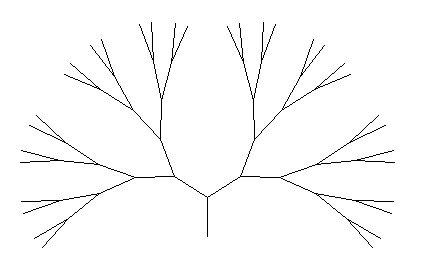
\includegraphics[scale=0.6]{parfait6}
\end{Exercise}
%--------------------------------------------------------------------------
%-------------------------------------------------------------------------------


%-------------------------------------------------------------------------------
%-------------------------------------------------------------------------------
\end{document}
%-------------------------------------------------------------------------------
%-------------------------------------------------------------------------------
%-------------------------------------------------------------------------------
%-------------------------------------------------------------------------------
%-------------------------------------------------------------------------------

